%%PREAMBLE %%%%%%%%%%%%%%%%%%%%%%%%%%%%
\documentclass[10pt, a4paper]{article}% size of txt = 10pt
\usepackage[top= 2cm,
			bottom = 2cm,
			left = 1.7cm,
			right = 1.7cm,
			footskip = 0.5cm,
			headsep = 0cm,
			headheight = 0cm
					]{geometry}
\usepackage{amsmath} % math packages
\usepackage{amsfonts}% math packages
\usepackage{amssymb} % math packages
\usepackage{graphicx} %package for including graphics
\usepackage{array}
\usepackage[thinlines]{easytable}
\usepackage{float}
\usepackage[section]{placeins}
\usepackage[hidelinks]{hyperref}
\usepackage[shortlabels]{enumitem}
\usepackage{svg}
\usepackage{bigstrut}
\usepackage{wrapfig,lipsum,booktabs}
\usepackage{subcaption}
\usepackage{xfrac}
\usepackage{pdfpages}
\usepackage{listings}
\usepackage{xcolor}
\usepackage{enumitem}
\usepackage{listings}
\usepackage{color} %red, green, blue, yellow, cyan, magenta, black, white
\definecolor{mygreen}{RGB}{28,172,0} % color values Red, Green, Blue
\definecolor{mylilas}{RGB}{170,55,241}

\definecolor{codegreen}{rgb}{0,0.6,0}
\definecolor{codegray}{rgb}{0.5,0.5,0.5}
\definecolor{codepurple}{rgb}{0.58,0,0.82}
\definecolor{backcolour}{rgb}{1,1,1}

\lstdefinestyle{mystyle}{
    backgroundcolor=\color{backcolour},   
    commentstyle=\color{codegreen},
    keywordstyle=\color{magenta},
    numberstyle=\tiny\color{codegray},
    stringstyle=\color{codepurple},
    basicstyle=\ttfamily\footnotesize,
    breakatwhitespace=false,         
    breaklines=true,                 
    captionpos=b,                    
    keepspaces=true,                 
    numbers=left,                    
    numbersep=5pt,                  
    showspaces=false,                
    showstringspaces=false,
    showtabs=false,                  
    tabsize=2
}
\lstset{style=mystyle}


%date format
\def\mydate{\leavevmode\hbox{\twodigits\day.\twodigits\month.\the\year}}
\def\twodigits#1{\ifnum#1<10 0\fi\the#1}

\usepackage{indentfirst}
\setlength{\parindent}{1cm}

\makeatletter
\newcommand{\thickhline}{%
    \noalign {\ifnum 0=`}\fi \hrule height 2pt
    \futurelet \reserved@a \@xhline
}
\newcolumntype{"}{@{\hskip\tabcolsep\vrule width 2pt\hskip\tabcolsep}}
\makeatother
\newcolumntype{?}{!{\vrule width 2pt}}
%%DOC ENVIROMENT%%%%%%%%%%%%%%%%%%%%%%%
\begin{document}
%Title 
\begin{flushleft}%% left justification
	\textbf{\Large{MKC-NBS: Úkol č. 3}}\hfill Filip Paul\\
	\large{ETHERNET, TCP, Firewall \hfill\mydate}
\end{flushleft}
\section*{\large{\textbf{Zapouzdřování datových jednotek protokolů}}}
	\begin{itemize}[label={}]
		\item \textbf{Zadání:}\\
		Níže je uveden výpis bajtů linkového rámce Ethernet II poskytnutý programem WireShark. V
		souladu se strukturou datových jednotek příslušných protokolů linkové, síťové a transportní vrstvy
		uveďte typ pole, do nichž jednotlivé bajty náleží (např. Toto pole reprezentuje MAC adresu
		zdroje) a vysvětlete význam konkrétní hodnoty pole, případně jednotlivých bitů pole (např. Tato
		hodnota bitu povoluje fragmentaci). Pole zprávy protokolu aplikační vrstvy vysvětlovat nemusíte\\\\

		 b8 af 67 f7 a8 ef 00 1f d0 39 cc ac 08 00 45 00 \\
		 00 3b 8d c8 40 00 40 11 aa bb 93 e5 93 59 93 e5 \\
		 47 0a b3 b5 00 35 00 27 38 69 e8 62 01 00 00 01 \\
		 00 00 00 00 00 00 03 77 77 77 06 73 65 7a 6e 61 \\
		 6d 02 63 7a 00 00 01 00 01 \\
		
		\item \textbf{Vypracování:}\\
		\begin{figure}[ht!]
			\centering
			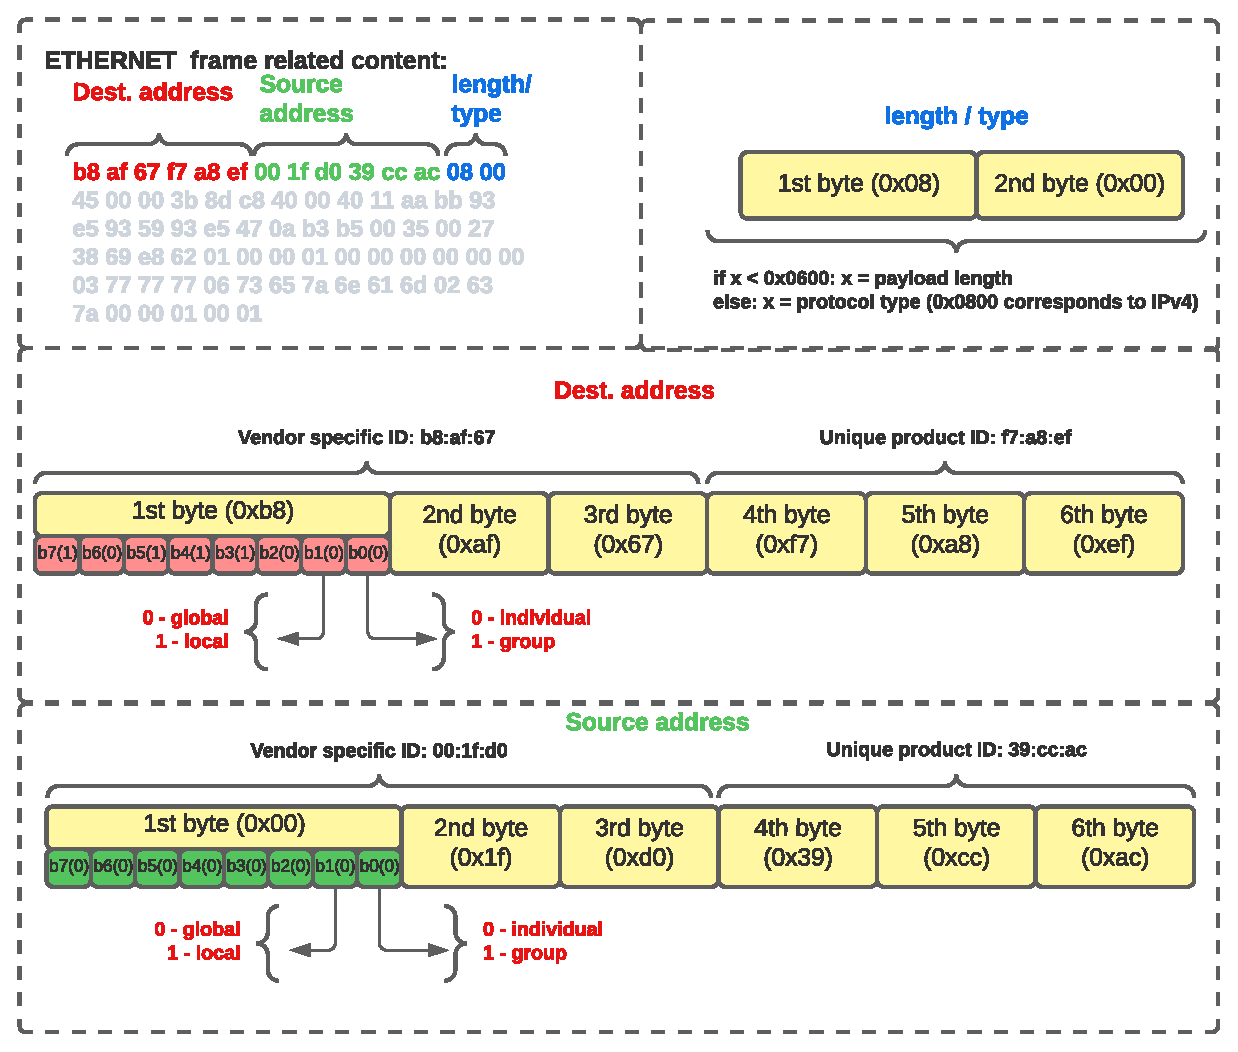
\includegraphics[width = 1\textwidth]{pictures/ETHERNET.eps}
		\end{figure}
		\clearpage
		\begin{figure}[ht!]
			\centering
			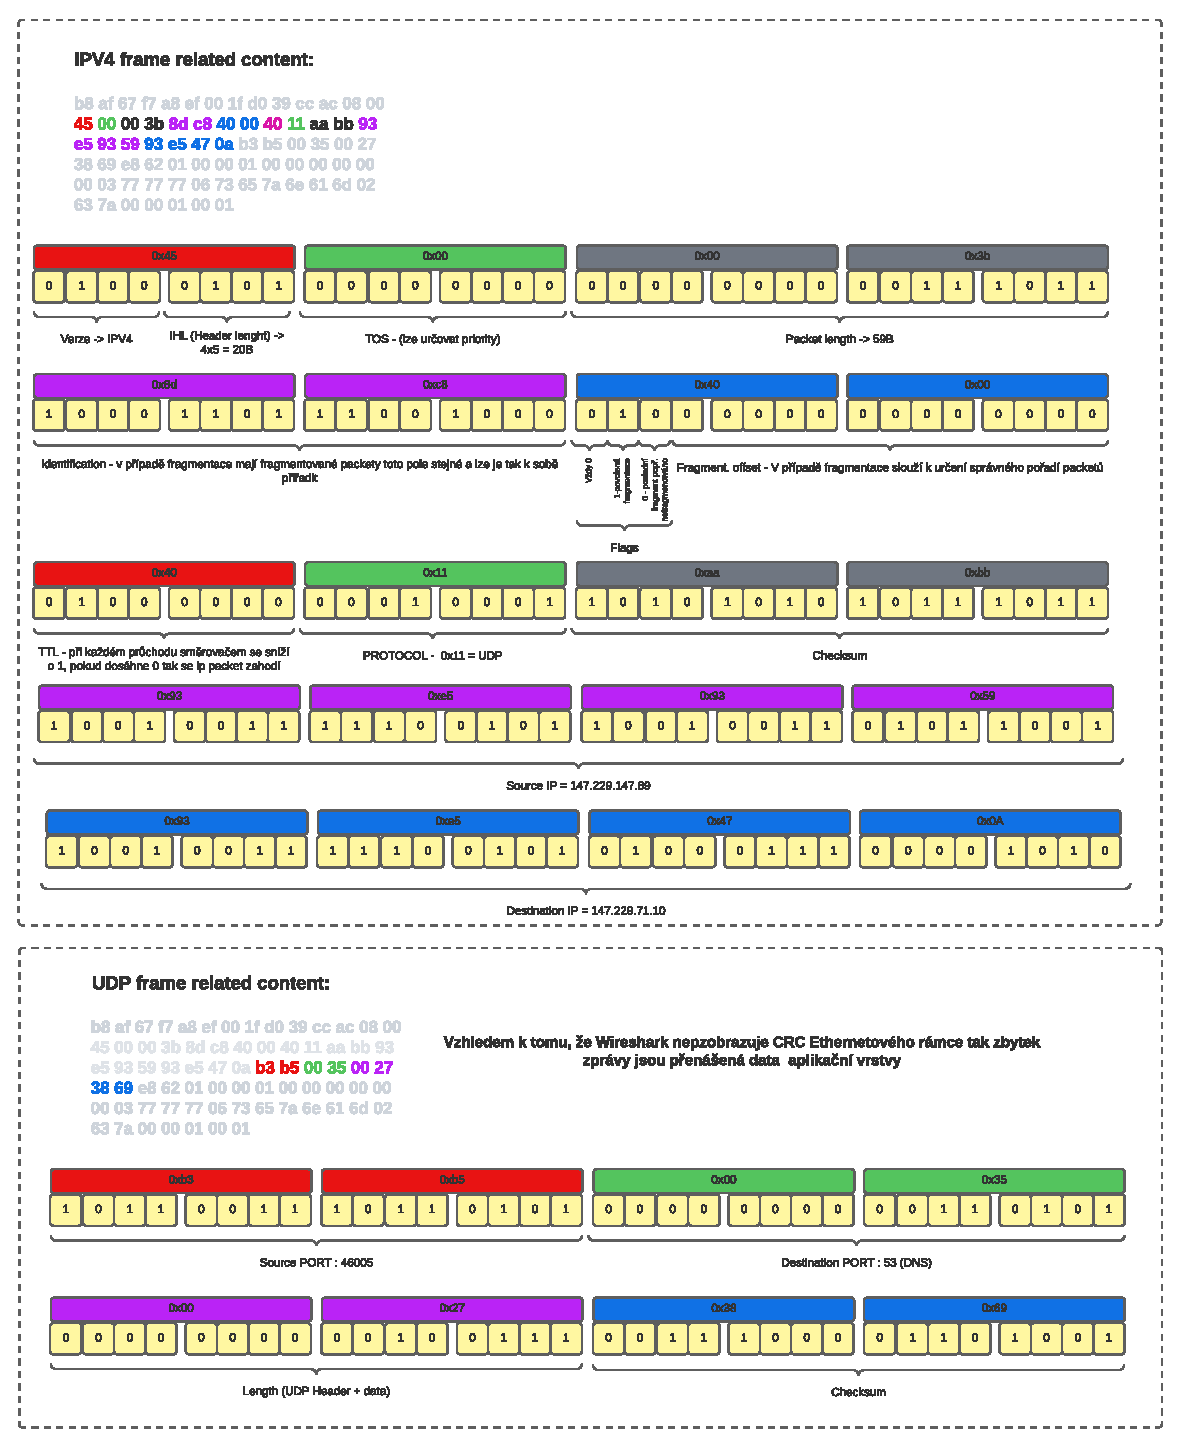
\includegraphics[width = 1\textwidth]{pictures/IPUDP.eps}
		\end{figure}

		\end{itemize}
	
		\clearpage
	\section*{\large{\textbf{ Protokol TCP}}}
		\begin{itemize}[label={}]
			\item \textbf{Zadání:}\\
			Níže je uveden výpis bajtů ze záhlaví jednoho segmentu protokolu TCP. Uveďte typ pole, do nichž
			jednotlivé bajty náleží (např. Příznaky) a vysvětlete význam konkrétní hodnoty (např. Tyto
			hodnoty signalizují příznak RST). Volitelné položky záhlaví vysvětlovat nemusíte.\\\\

			 01 bb 04 b9 5f e0 24 ab 44 74 21 96 60 12 fa f0 \\
			 1d 1e 00 00 02 04 05 b4 


			\item \textbf{Vypracování:}\\
			\begin{figure}[ht!]
				\centering
				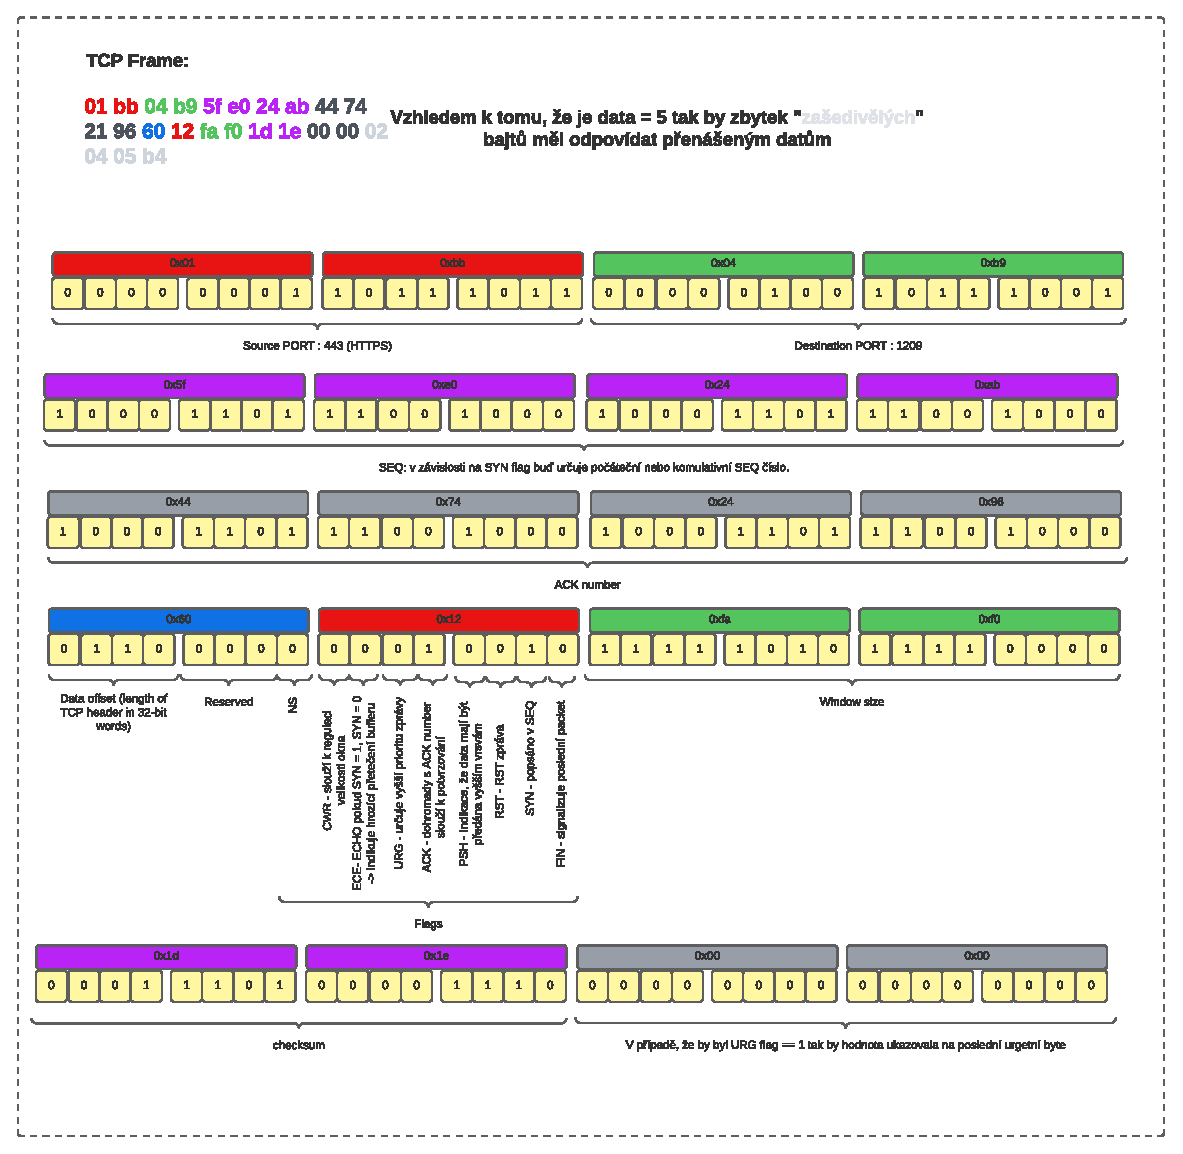
\includegraphics[width = 1\textwidth]{pictures/TCP.eps}
			\end{figure}
		\end{itemize}
		\clearpage
	\section*{\large{\textbf{Firewal se stavovou inspekcí}}}
		\begin{itemize}[label={}]
			\item \textbf{Zadání:}\\
			Firewal se stavovou inspekcí propustil z vnitřní sítě do vnější sítě paket P1 s následujícími
			parametry: \\
			\begin{itemize}
				\item zdrojová IP adresa ZA1 = 172.16.73.73, cílová IP adresa CA1 = 63.245.132.132,
				\item IP číslo protokolu C1 = 6 (tj. TCP),
				\item zdrojový port ZP1 = 04B9, cílový port CP1 = 01BB,
				\item číslo SN1 = 6DD61879, číslo AN1 = 00000000,
				\item příznaky P1 = SYN, délka dat L1 = 0 B.\\\\
				Z vnější sítě byl nyní doručen paket P2 s parametry: 
				\item zdrojová IP adresa ZA2 = 63.245.132.132, cílová IP adresa CA2 = 172.16.73.73,
				\item IP číslo protokolu C2 = 6 (tj. TCP),
				\item zdrojový port ZP2 = 01BB, cílový port CP2 = 04B9,
				\item číslo SN2 = 10423A61, číslo AN2 = 6DD6187A,
				\item příznaky P2 = SYN+ACK, délka dat L2 = 0 B.
			\end{itemize}


			Náš stavový firewal kontroluje soulad hodnot všech výše uvedených parametrů. Bude paket P2 
			vpuštěn do vnitřní sítě, či nikoliv? A proč 


			\item \textbf{Vypracování:}\\
			Protože sedí cílové a zdrojové adresy a porty, AN2 se rovná SN1 + 1,tak by měl Firwall packet propustit.
			Nicméně nesmí být blokována CA1 a ZP1 v cílových adresách filtrační tabulky. Nejsem si však jistý, zda tuto
			podmínku už neřeší Firewall se stavovou inspekcí při odesílání packetu P1.

		\end{itemize}

\end{document}